\section{\Glsfmtlong{cnn}}
\label{sec.cnn}

En dépit d'être une architecture naturelle pour le traitement des séquences,
les \glspl{rnn} sont trop lents pour la majorité des cas d'utilisation pratiques.
Cela est dû à leur nature séquentielle qui à son tour, 
est due à leur utilisation de boucles de rétroaction (Voire Section~\ref{sec.rnn}).
Une architecture sans telles boucles (i.e une architecture d'\gls{ffn}) est donc préférable.

Les \glspl{cnn} sont une famille d'\glspl{ffn} typiquement utilisés en traitement d'images.
Ils ont été introduits par~\cite{Fukushima_1980} et popularisés par%
~\cite{LeCun_Boser_Denker_Henderson_Howard_Hubbard_Jackel_1989,Lecun_Bottou_Bengio_Haffner_1998}.
Les \glspl{cnn} atteignent des performances comparables à celles des \glspl{rnn} sans mémoire explicite.
Ils y parviennent en exploitant un outil mathématique appelé produit de \emph{convolution}%
~\cite{Calin_2020}.

\subsubsection{Principes mathématiques de fonctionnement}

Le produit de convolution de deux signaux \(f\) et \(g\) est le signal \(f \ast g\) donné par
\begin{equation}
    \label{eq.convolution}
    u \mapsto \int_\reals f(u-t)g(t)\diff{t}
\end{equation}
il s'agit d'une opération commune en probabilité, analyse fonctionnelle, 
traitement de signaux et traitement d'images~\cite{Barbe_Ledoux_2012,Oppenheim_Schafer_2013}.
À partir d'elle, une autre opération appelée \emph{l'inter-corrélation} est définie.
L'inter-corrélation de \(f\) et \(g\) est notée \(f\star g\).
Elle est définie par
\begin{equation}
    \label{eq.cros-corr}
    u \mapsto \int_\reals f(t)g(t-u)\diff{t} = (f \ast g^-)(u)
\end{equation}
ou \(g^- : t \mapsto g(-t)\).
Intuitivement, elle mesure la similarité entre les deux signaux en question.
Les \glspl{cnn} utilisent l'inter-corrélation à la place des applications linéaires quelconques d'un \gls{mlp}.
Une couche de convolution unidimensionnelle calcul donc la fonction suivante
\begin{equation}
    \label{eq.layer-conv1d}
    x \mapsto \phi\left(b + \sum_{i=1}^n x\star w_i\right)
\end{equation}
ou \(x\) est l'entrée et les vecteurs \(w_i\) sont les paramètres entraînables de la couche, 
aussi appelés ses \emph{noyaux} ou \emph{masques}
(Voire Figure~\ref{fig.layer-conv1d}).
La sortie de cette couche est une combinaison de tous les éléments de la séquence d'entrée.
En composant suffisamment de telles couches,
un \gls{cnn} apprend une représentation de l'entrée beaucoup plus structurée qu'un \gls{mlp}.
On parle par fois de représentation \emph{hiérarchique}.

\begin{figure}[hbt]
    \begin{center}
        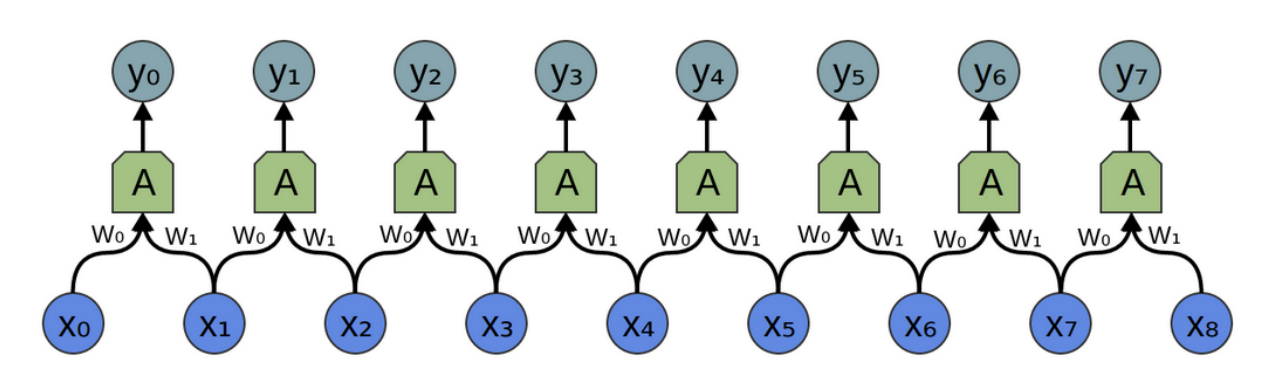
\includegraphics[width=\textwidth]{assets/images/conv1d.png}
    \end{center}    
    \caption{Couche convolutive unidimensionnelle.}
    \label{fig.layer-conv1d}
\end{figure}


\subsubsection{Application à l'apprentissage \glsfmtshort{s2s}}

Leur tendance naturelle à produire des représentations synthétiques des entrées,
fait des \glspl{cnn} des encodeurs très puissants pour une grande variété de tâches,
y compris des tâches de transduction de séquences.
Plusieurs travaux ont combiné un encodeur convolutif avec un décodeur récurrent%
(Voire~Figure~\ref{fig.rctm}, \barecite[Fig.3]{Kalchbrenner_Blunsom_2013})%
~\cite{deep-nmt-survey}.

\begin{figure}[hbt]
    \centering
    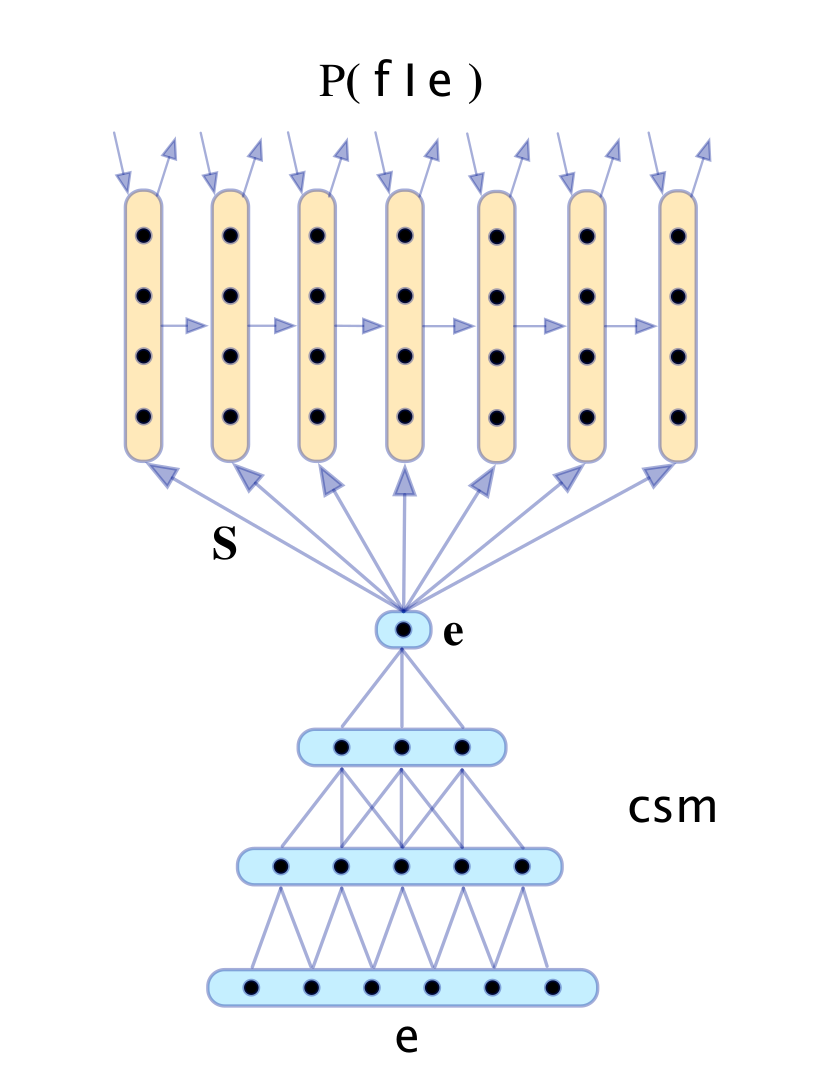
\includegraphics[width=6cm]{assets/images/ctrm.png}
    \caption{Recurrent Continuous Translation Model}
    \label{fig.rctm}
\end{figure}

Cependant, des architectures totalement convolutives pour l'apprentissage \gls{s2s} existent également.
ByteNet (Voire Figure~\ref{fig.bytenet}
\barecite{Kalchbrenner_Espeholt_Simonyan_Oord_Graves_Kavukcuoglu_2017})
et ConvS2S (Voire Figure~\ref{fig.convs2s}
\barecite{Kameoka_Tanaka_Kwaśny_Kaneko_Hojo_2020})
sont deux exemples de telles architectures.

\begin{figure}[H]
    \centering
    \begin{minipage}{.5\linewidth}
        \centering
        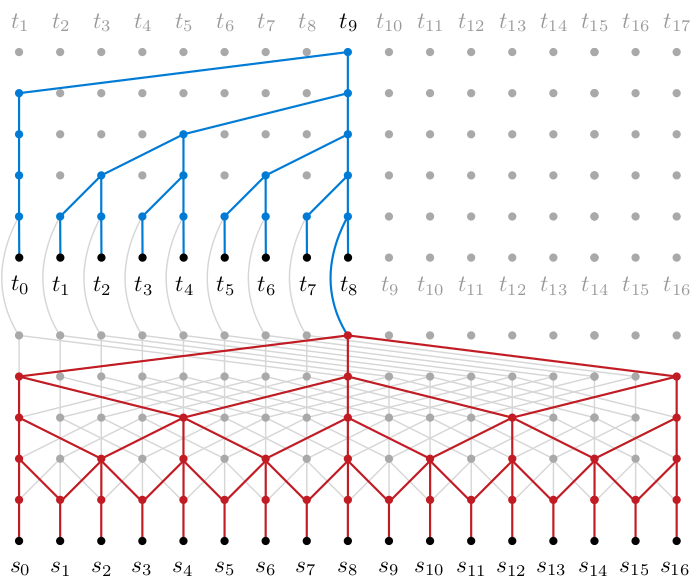
\includegraphics[height=5cm]{assets/images/bytenet.png}
        \captionof{figure}{Architecture de ByteNet.}
        \label{fig.bytenet}
    \end{minipage}%
    \begin{minipage}{.5\linewidth}
        \centering
        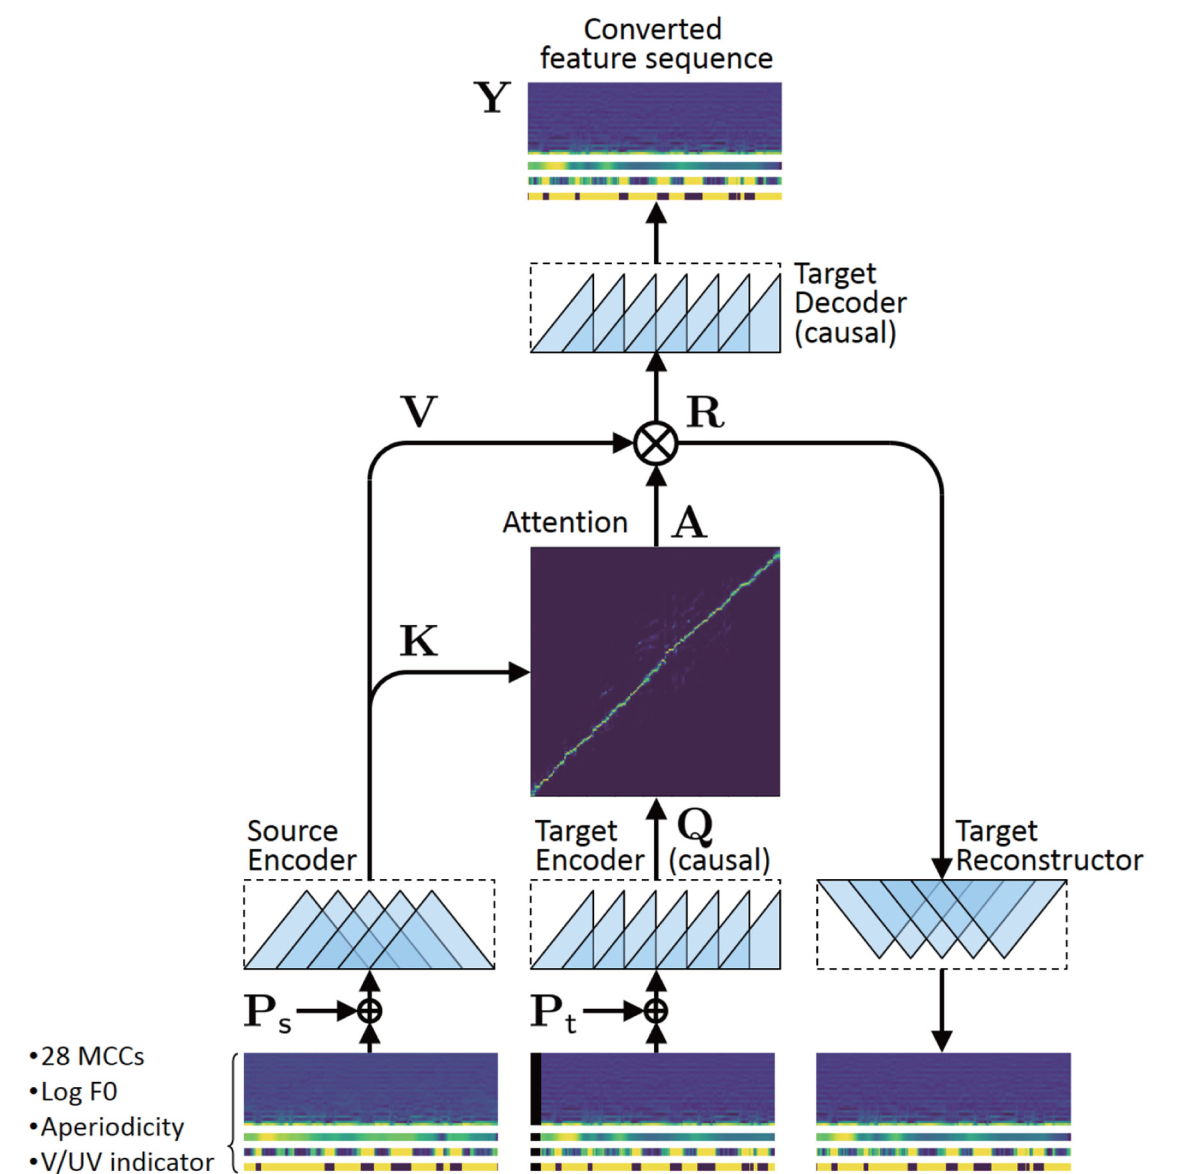
\includegraphics[height=5cm]{assets/images/convs2s.png}
        \captionof{figure}{Architecture de ConvS2S.}
        \label{fig.convs2s}
    \end{minipage}
\end{figure}


\subsubsection{Avantages et inconvénients}

Le produit de convolution (et par conséquent, inter-corrélation) 
est une opération très facile à paralléliser.
Il est donc possible d'exploiter des architectures matérielles parallèles (GPU) 
pour accélérer l'entraînement des \glspl{cnn}.
À cet effet, les \glspl{cnn} sont beaucoup plus efficaces que les \glspl{rnn} pour les entrées longues. 
Ils peuvent être employés dans des cas pratiques de tailles raisonnables%
~\cite{Li_Zhang_Huang_Wang_Zheng_2016}.

Or, la nature locale du produit de convolution
rend difficile aux \glspl{cnn} d'apprendre les corrélations globales%
\footnote{Dépendances entre des couples d'éléments éloignés dans la séquence}.
En effet, pour représenter toutes les relations dans une séquence de longueur \(n\),
un \gls{cnn} dont les masques sont de taille \(k < n\) doit avoir \(\log_k n\) couche%
~\cite{attention}.
Le traitement de séquences très longues nécessite alors des \glspl{cnn} trop profonds,
cequi donne lieu au problèmes de dispartion et d'exploision des gradients.